
\title{Deep Learning Project 1}
\author{
        Pranav A (20478966) \\
        Big Data Institute\\
        Hong Kong University of Science and Technology
}
\date{\today}

\documentclass[12pt]{article}
\usepackage{graphicx}
\usepackage{booktabs}
\usepackage{cite}
\begin{document}
\maketitle

\begin{abstract}
In this project, I have used logistic regression and multilayer perceptron as the classification of the data points.
At the end, two-layered multilayer perceptron outperformed than linear regression, achieving an accuracy of 97.3\% on the validation set.
However, the multilayer perceptron was overfitting before converging completely due to its complex architecture.
\end{abstract}

\section{Introduction}
Logistic regression is the most straightforward way to do classification.
This is visualized as the weighted-sum of the features to produce the best output.
This can also be thought of as a multilayer perceptron with no hidden layers.

MLP (Multilayer perceptron)  is the most fundamental forms of the artificial neural networks.
MLP introduces non-linearity through activation functions and extra layers to produce complex decision boundaries.

In this project, I have used these two techniques on the provided dataset.

\section{Experimental Setup}
The dataset comprises of 57 features with around 3220 items.
Since MLP are prone to overfitting, I have divided the dataset into traning and validation sets.
The training set comprises of 3000 items and the validation sets uses 220 items.

I have used Pytorch \cite{paszkepytorch} for developing this MLP architecture.

For logistic regression, I have used no hidden layers.
Thus the problem of MLP reduces down to just logistic regression.
Then I used Stochastic Gradient Descent, with a batch size of 128 and learning rate of 0.001.
Finally I used Cross-Entropy loss function with softmax as the output.

To generate a learning curve, at every iteration I plotted the loss and accuracy for training and validation set.

For multilayer perceptron, I have used two hidden layers.
Both hidden layers contain 64 neurons.
I have used Adam \cite{kingma2014adam} as the optimizer, with a batch size of 128 and learning rate of 0.001.
The activation functions used were Rectified Linear Units (ReLUs) \cite{dahl2013improving} at every layer (expect the output one).
Finally I used Cross-Entropy loss function after taking softmax of the output.

\section{Final Remarks}

\begin{figure}[]
	\centering
	\begin{minipage}{0.5\textwidth}
		\centering
		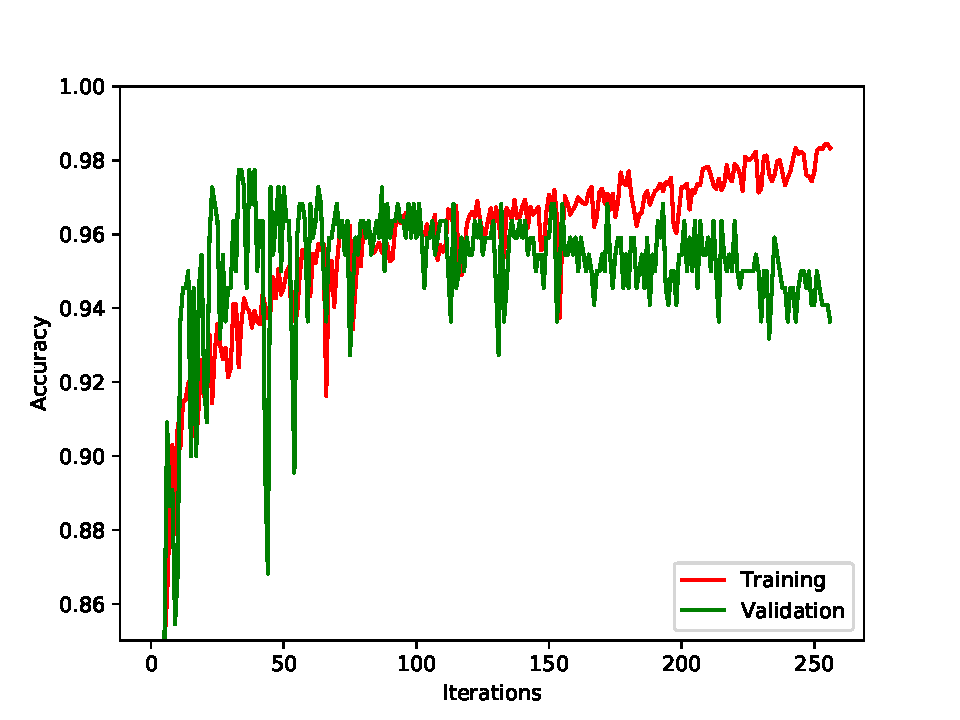
\includegraphics[width=1.1\textwidth]{Accuracy-Learning-Curve.pdf} % first figure itself
	\end{minipage}\hfill
	\begin{minipage}{0.5\textwidth}
		\centering
		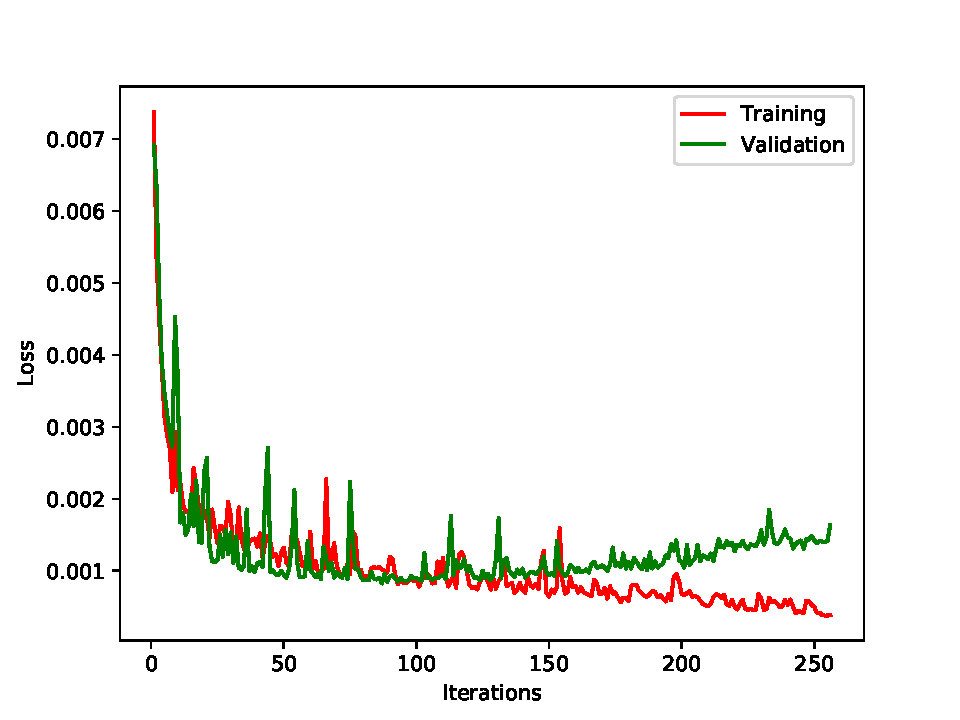
\includegraphics[width=1.1\textwidth]{Loss-Learning-Curve.pdf} % second figure itself
	\end{minipage}
	\caption{Plots of the learning curve for the 2-layers MLP. On the left, accuracy is plotted while on the right, loss is plotted}
\end{figure}

\begin{table}[h]
	\centering
	\label{my-label}
	\begin{tabular}{@{}lcc@{}}
		\toprule
		& Training Accuracy & Validation Accuracy \\ \midrule
		Logistic Regression & 89.6\%           & 87.2\%             \\
		MLP with 2 layers   & \textbf{98.4\%}  & \textbf{97.3\%}    \\ \bottomrule
	\end{tabular}
	\caption{Accuracy results of the algorithms}
\end{table}

The results are shown in Table 1.
Clearly, MLP with 2 layers performs better than Logistic Regression.
I have also plotted the learning curves of the MLP experiment in the figure 1.


From the figures it is easy to see that model has not fully converged but starts to overfit after 150 iterations.
This is due to no regularization has been applied to the MLP architecture.
Maybe, a less complex MLP with less layers and dropout would have resulted in a better performance without being prone to overfitting.

\bibliographystyle{apalike}
\bibliography{ref}
\end{document}
